\chapter{Data Types}

You have to specify the type of variables when initializing them in C++. Each variable can only be used to store data of a single type.\footnote{Out of scope: this is what we call a strongly typed language} These are also the available types for function arguments and function return values.

\section{Primary data types}
\label{sec:primarydtypes}
\textbf{Primary data types}\index{Primary data types} are those that are not composed of other data types. It is important to distinguish primary data types with other data types (like arrays), as we will see in \cref{sec:passbyref}

Some basic knowledge on bits and bytes $-$ 1 bit is a single 0 or 1 in memory, 8 bits form 1 byte, we usually discuss memory in terms of bytes instead of bits.

\begin{table}[h]
    \centering
    \begin{tabular}{|m{6em}|m{6em}|m{10em}|m{12em}|}
        \hline
        \textbf{Data Type} & 
        Bytes in Memory & 
        Range & 
        Remarks 
        \\ \hline \hline
        
        \texttt{int} &
        4 & 
        $-2^{31}$ to $2^{31}-1$ (i.e. -2147483648 to 2147483647) &
        
        \\ \hline
        
        \texttt{bool} &
        1 & 
        \texttt{true} / \texttt{false}  &
        \tablefootnote{Out of scope: in C++ bool is a primary data type, in C you will have to include stdbool.h to use it.} 
        \\ \hline
        
        \texttt{char} &
        1 & 
        /  &
        Stored using an integer, the ASCII code of the character
        \\ \hline
        
        \texttt{float} &
        4 &
        A large range \textcolor{gray}{ (~$-10^{38}$ to $10^{38}$)} &
        Stores numbers with decimal places
        \\ \hline
        
        \texttt{double} &
        8 & 
        A large range \textcolor{gray}{ (~$-10^{308}$ to $10^{308}$)} &
        Stores numbers with decimal places
        \\ \hline
    \end{tabular}
\end{table}

\pagebreak

These are variants of integers. They are of less importance.\footnote{Reference: \href{https://en.cppreference.com/w/cpp/language/types}{https://en.cppreference.com/w/cpp/language/types}, the range and bytes occupied differs for different version of C++}

\begin{table}[h]
    \centering
    \begin{tabular}{|m{6em}|m{6em}|m{10em}|m{12em}|}
        \hline
        \textbf{Data Type} & 
        Bytes in Memory & 
        Range & 
        Remarks 
        \\ \hline \hline
        
        \texttt{unsigned} &
        4 & 
        $0$ to $2^{32}-1$ (i.e. 0 to 4294967295) &
        Cannot store negative numbers, yet approximately double the range.
        \\ \hline
        
        \texttt{short} &
        2 & 
        $-2^{15}$ to $2^{15}-1$ (i.e. -32768 to 32767) &
        Half the size of an \texttt{int}
        \\ \hline
        
        \texttt{long long} &
        8 & 
        $-2^{63}$ to $2^{63}-1$ &
        Double the size of an \texttt{int}
        \\ \hline
        
    \end{tabular}
\end{table}

\section{Integer overflow\index{overflow}}

As you saw in \cref{sec:primarydtypes}, integers have a limited range. Overflow occurs when the value we want to store is out of the range that the data type can represent. 

For integers (\texttt{int}, \texttt{unsigned}, \texttt{short}, \texttt{long long}), the value it represents will go to the other end of the range when they overflow.\footnote{Reason behind out of scope: requires understanding of two's compliment}. 

For example,
\begin{lstlisting}
int x = 2147483647;
cout << "Before overflow: " << x << endl; //2147483647
x += 1;
cout << "After overflow: " << x << endl; //-2147483648

unsigned y = 4294967295;
cout << "Before overflow: " << y << endl; //4294967295
y += 1;
cout << "After overflow: " << y << endl; //0
\end{lstlisting}

\section{Floating point values}

OK, the range of floating point values\index{floating point values} (\texttt{float} and \texttt{double}) are much larger than ints, so is it a good idea to use them all the time? NO!

Floating point values store values inaccurately, and \textbf{rounding errors} accumulate. Even though using \texttt{double} reduces the rounding error, floating point values are still nasty in some ways. 

You are advised to only use \texttt{double} to store numbers with decimal points and very large numbers (those can't be represented by \texttt{long long}). And never use \texttt{float}\footnote{Memory usage is not a problem nowadays}.

\section{Boolean operators}

A Boolean\index{Boolean} variable (\texttt{bool}) can be either \texttt{true} or \texttt{false}. There are three operations that we can perform on \texttt{bool}s. Including AND (\&\&), OR (\textbar\textbar), NOT (!).

\begin{table}[h]
    \centering
    \begin{tabular}{|m{4em}|m{4em}|m{4em}|m{4em}|m{4em}|}
        \hline
        a & 
        b & 
        a \&\& b & 
        a\textbar\textbar b & 
        !a 
        \\ \hline \hline
        
        true & 
        true & 
        true & 
        true & 
        false 
        \\ \hline
        
        true & 
        false & 
        false & 
        true & 
        false 
        \\ \hline
        
        false & 
        true & 
        false & 
        true & 
        true 
        \\ \hline
        
        false & 
        false & 
        false & 
        false & 
        true 
        \\ \hline
        
    \end{tabular}
\end{table}

C/C++ recognizes 0 as false and other non-zero values as true. It is common to use 1 instead of true\footnote{a convention} and 0 instead of false.

You could do \texttt{while(true) ...} for an infinite loop, but you might as well do \texttt{while(1) ...}
\vspace{6mm}

Order of precedence: ! $>$ \&\& $>$ \textbar\textbar

For example, 

!0 \textbar\textbar 0 \&\& 1

= (!0) \textbar\textbar 0 \&\& 1

= 1 \textbar\textbar 0 \&\& 1

= 1 \textbar\textbar (0 \&\& 1)

= 1 \textbar\textbar 0

= 1

\subsection{Bitwise operators}

\textit{Difficult topic}
\vspace{6mm}

Don't have time to cover, there should be plenty of resources online on this topic. 

Yet, it is important for senior group contestants as this kind of questions seem common. 

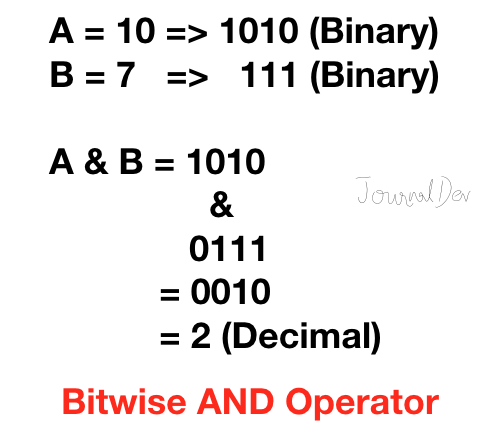
\includegraphics[width=7cm]{ch3-bitwise.png}
\footnote{Reference: \href{https://www.digitalocean.com/community/tutorials/python-bitwise-operators}{https://www.digitalocean.com/community/tutorials/python-bitwise-operators}}

\section{Characters are integers}

Let's run some C++ code.

\begin{lstlisting}
char a = 'a'; //we use single quotes for characters and double quotes for strings
printf("%d %c\n",a,a); //97 a
a = 97;
printf("%d %c\n",a,a); //97 a
a = 65;
printf("%d %c\n",a,a); //65 A
a += 1;
printf("%d %c\n",a,a); //66 B
\end{lstlisting}

It seems that each character is associated with an integer. That's right! 128 (later extended to 256) frequently used characters are chosen (including the English letters, digits, and common symbols) and they are associated with an integer between 0 and 127.\footnote{ASCII Table: \href{https://simple.wikipedia.org/wiki/ASCII}{https://simple.wikipedia.org/wiki/ASCII}}

We can perform arithmetic operations with \texttt{char} variables, as they are just integers! 

\section{Type casting}

We can covert values from one type to another, by putting the target type, enclosed with parenthesis, on the left of the value.

\begin{lstlisting}
cout << (int) 40.9 << endl; //40
cout << (bool) -1 << endl; //1
cout << (int) 'a' << endl; //97
\end{lstlisting}

When floating point values are cast to an integer, it is \textbf{rounded down}. Non-zero values are cast to \texttt{true}, hence \texttt{1} is displayed. The character \texttt{a} is converted to an integer based on its ASCII code.

Type cast is done automatically whenever possible\footnote{When it is not possible, e.g. from integer array to character, an error would occur} when a value is assigned to a variable of a different type. Note that type of a variable cannot be changed. 

\begin{lstlisting}
int x;
x = 40.9; //x is an int, so 40.9 got cast into an integer, 40, before storing into x
cout << x << endl; //40
\end{lstlisting}

\section{Strings}

\textit{Of less importance, except operation on string variables}
\vspace{6mm}

Strings are best understood as an array of characters, we would store them using a character array such as  \texttt{char s[10] = "Hello";} \footnote{We would avoid using the type \texttt{string} in C++, but use character arrays to store strings}, but there are a few nasty catches.

\subsection*{Strings terminate with a null character \texttt{\textbackslash 0}}

Hm, the word \texttt{hello} only has 5 characters, can we do \texttt{char s[5] = "Hello";} instead? Not really.

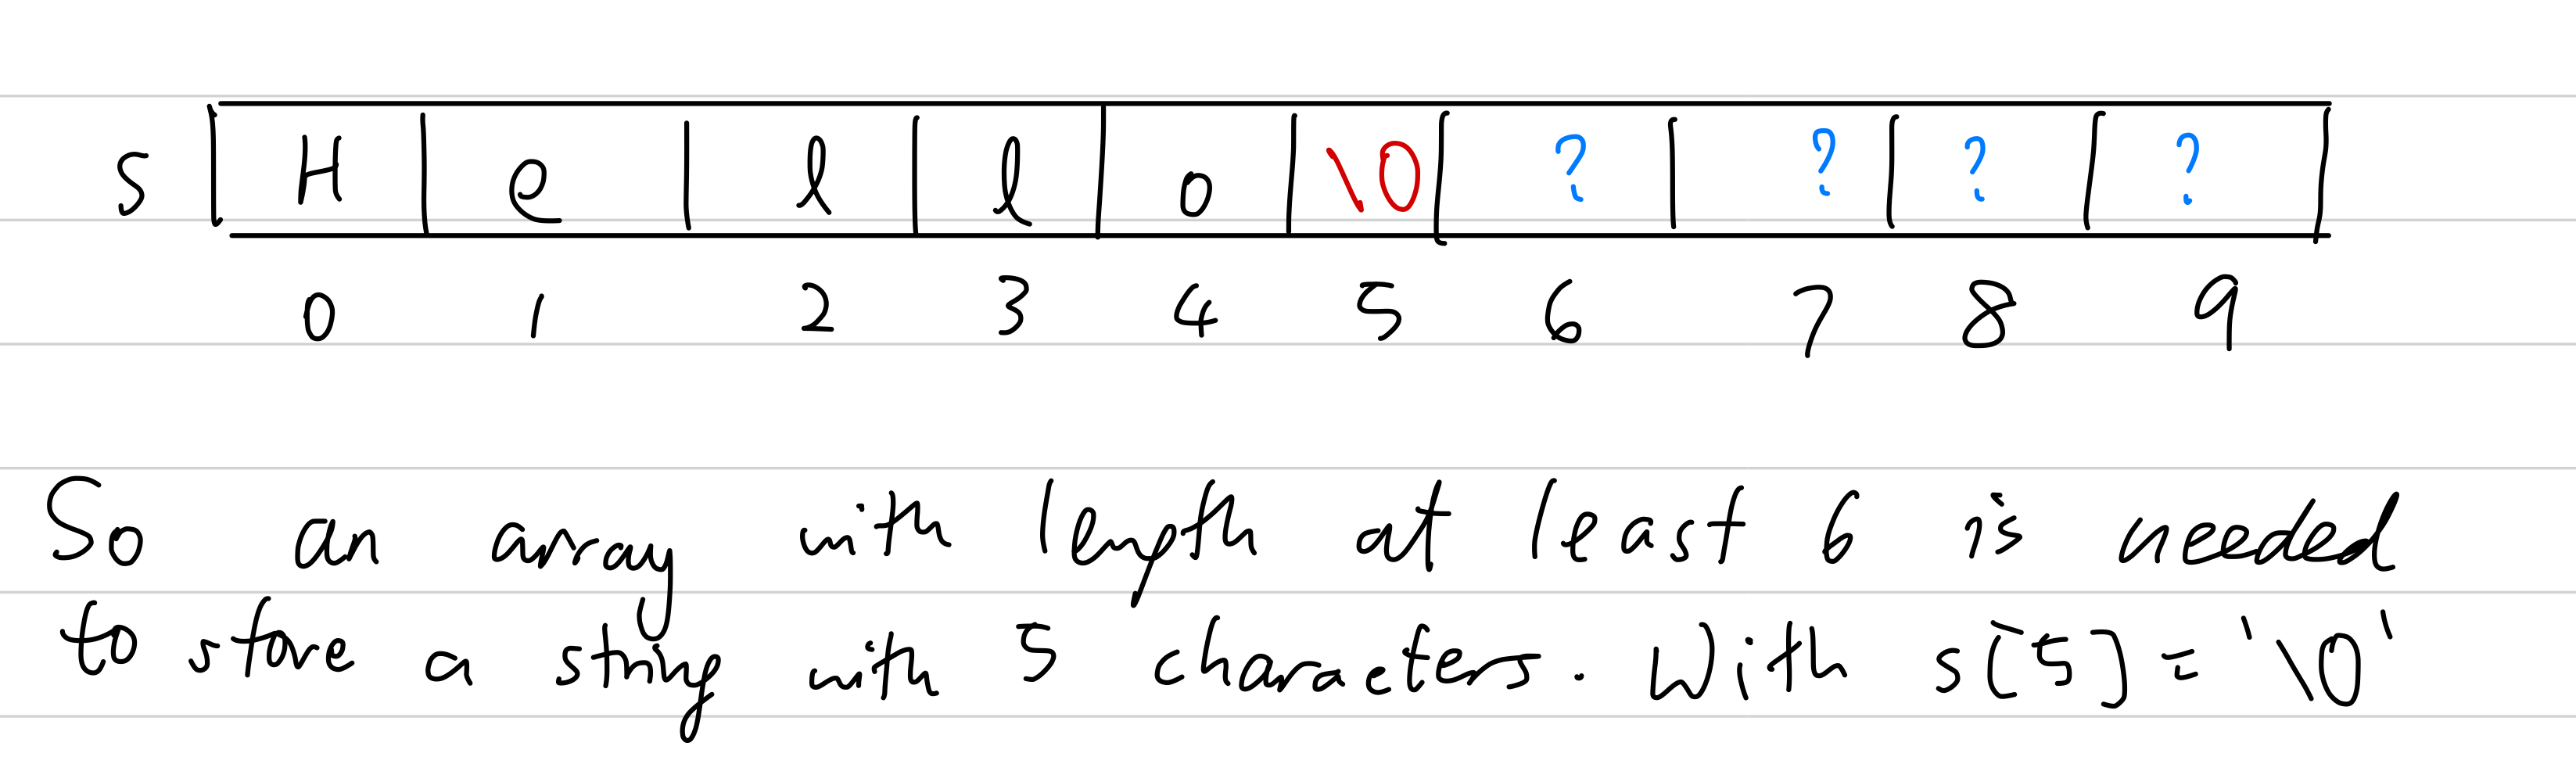
\includegraphics[width=15cm]{ch3-nullstring.png}

The \texttt{\textbackslash 0} (ASCII code = 0) indicates the end of a string, it is necessary for C/C++ programs so that they could identify when the string ends. If you remove it something bad would happen...

Don't trust me? Try running:

\begin{lstlisting}
char s[4] = "FGH";
s[3] = 'I'; //Remove the \0 character and replace it by character I
cout << s << endl; //FGHI followed by a bunch of nonsense, the nonsense is different everytime we run the program

char s1[7] = { 'A', 'B', 'C', '\0', 'D', 'E', '\0'};
cout << s1 << endl; //ABC
\end{lstlisting}

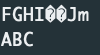
\includegraphics[width=3cm]{ch3-beyondnull.png}

The first example shows what happens when we explicitly remove the null character at the end of the string. (By replacing \texttt{FGH\textbackslash 0} with \text{FGHI}) It attempts to access and print things beyond the memory allocated. (see chapter 5 for more details)

The second example verifies that the null character is recognized by C/C++ as the end of the string, despite having some other contents after the null character.

\textbf{So we always have to reserve one more space for the null character.}

\subsection*{\texttt{cin} obtains input word by word}

This example shows that \texttt{cin} only catches the first word and store it in \texttt{s2}, while leaving other words for future calls of \texttt{cin}.

\begin{lstlisting}
char s2[20], s3[20];
cin >> s2; //You inputted Hello world
cout << s2 << endl; //Hello

cin >> s3; //The computer did not ask for your input
cout << s3 << endl; //world
\end{lstlisting}

\label{sec:cingetline}
However, sometimes you want to obtain a whole line of text input rather than just a word. You could use \texttt{cin.getline}. It accepts two arguments, first the string variable (the character array you defined), second the maximum amount of characters it should get (you have to set it less than or equal to the size of the chracter array)

\begin{lstlisting}
char s4[20];
cin.getline(s4,20); //You inputted Good morning
cout << s4 << endl; //Good morning
\end{lstlisting}

Unfortunately it is not as simple as that, things get complicated when you have other \texttt{cin}s in the same program.

\begin{lstlisting}
char s2[20], s3[20];
cin >> s2; //You inputted Hello world
cout << s2 << endl; //Hello

cin >> s3; //The computer did not ask for your input
cout << s3 << endl; //world

char s4[20];
cin.getline(s4,20); //The computer did not ask for your input
cout << s4 << endl; //Probably a next line symbol (\n)
\end{lstlisting}

This behaviour is probably\footnote{Who is certain about this chaos?} due to the next line symbol of the Hello world line has not been read (\texttt{\textbackslash n} is inputted when you press enter to confirm your input), and \texttt{cin.getline} reads the text until it hits a next line symbol, and that is the only thing stored in \texttt{s4}.

What you could do is use \texttt{cin.clear()} and \texttt{cin.ignore(10000,'\textbackslash n')} (both are required) before \texttt{cin.getline}, in order to clear the buffer.

\begin{lstlisting}
char s2[20], s3[20];
cin >> s2; //You inputted Hello world
cout << s2 << endl; //Hello

cin >> s3; //The computer did not ask for your input
cout << s3 << endl; //world

char s4[20];
cin.clear();
cin.ignore(10000, '\n');
cin.getline(s4,20); //You inputted Good morning
cout << s4 << endl; //Good morning
\end{lstlisting}

Alternatively, you could call \texttt{cin.getline} twice, the first one to read the previous line, and the second one to actually read your input. The result of the first read is overwritten by the second one as desired.

\begin{lstlisting}
char s2[20], s3[20];
cin >> s2; //You inputted Hello world
cout << s2 << endl; //Hello

cin >> s3; //The computer did not ask for your input
cout << s3 << endl; //world

char s4[20];
cin.getline(s4,20); //read the previous line
cin.getline(s4,20); //You inputted Good morning
cout << s4 << endl; //Good morning
\end{lstlisting}

\subsection{Strings VS string variables}

The following two restrictions concern string variables but not strings. Now let's differentiate strings and string variables.
\vspace{6mm}

Strings are hard coded in the source code, only for one time use. Normal users (not you, you are the programmer) cannot change it.

String variables are character arrays that are used to store strings. They can be changed by users if their values are obtained by input, e.g. \texttt{cin}. 

\subsection*{String variables cannot be compared normally}

You can compare them normally using comparison operators.

\begin{lstlisting}
cout << ("ABC"=="DEF") << endl; //0
cout << ("ABC" < "DEF") << endl; //1 (why?)
cout << ("abc" <= "ABC") << endl; //0 (why?)
\end{lstlisting}

Sadly they return unmeaningful results when string variables are being compared. (use strcmp instead)\footnote{Reason out of scope: because the references of the arrays are compared instead of their values. You may understand more in Chapter 5 but the full concept is not necessary}

\begin{lstlisting}
char s5[20] = "ABC", s6[20] = "ABC", s7[20] = "DEF";
cout << (s5==s5) << endl; //1
cout << (s5==s6) << endl; //0
cout << (s5<s6) << endl; //0
\end{lstlisting}

Use \texttt{strcmp} instead (will be formally introduced next section)
\begin{lstlisting}
char s8[20] = "ABC", s9[20] = "ABC", s10[20] = "DEF";
cout << strcmp(s8,s9) << endl; //0, implying s8 equals s9
cout << strcmp(s8,s10) << endl; //negative value, implying s8 < s10
\end{lstlisting}

\subsection*{The whole string variable cannot be reassigned}

Thought you could do this? Nah...

\begin{lstlisting}
char s11[20] = "ABCD";
s11 = "XYZ"; //SYNTAX ERROR
\end{lstlisting}

Well you could do the following instead if you are desperate, but it is much better using \texttt{strcpy} (will be formally introduced next section)

\begin{lstlisting}
//desperate way:
s11[0] = 'X'; 
s11[1] = 'Y'; 
s11[2] = 'Z'; 
s11[3] = '\0'; 

//better way:
strcpy(s11,"PQR");
\end{lstlisting}


\subsection{Operation on string variables (IMPORTANT)}

\begin{lstlisting}
#include <cstring>
\end{lstlisting}

\begin{table}[h]
    \centering
    \begin{tabular}{|m{9em}|m{25em}|}
        \hline
        \textbf{Function} & 
        Usage 
        \\ \hline \hline
        
        \texttt{strlen(s)} &
        Get string length
        \\ \hline
        
        \texttt{strcpy(s1, s2)} &
        Copy value stored in \texttt{s2} to \texttt{s1} 
        \\ \hline
        
        \texttt{strcat(s1, s2)} &
        Concatenate (i.e. combine) the two strings, store it in \texttt{s1} 
        \\ \hline
        
        \texttt{strcmp(s1, s2)} &
        Compare two strings, returns 0 if \texttt{s1} = \texttt{s2}, returns a negative number if \texttt{s1} $<$ \texttt{s2}, returns a positive number if \texttt{s1} $>$ \texttt{s2}. (In dictionary order with respect to ASCII code)
        \\ \hline
    \end{tabular}
\end{table}

You are advised to try out these operations yourself, I am sure you will find surprises.

\section{Conclusion and further resources}

\href{https://www.youtube.com/watch?v=Zy2bNkSxv8M}{This video}\footnote{Link: \href{https://www.youtube.com/watch?v=Zy2bNkSxv8M}{https://www.youtube.com/watch?v=Zy2bNkSxv8M}} summarizes some more nasty things about strings. Bear in mind what you can and what you can't do with them.
\vspace{6mm}

\begin{center}
\textit{The most comfortable type to deal with are integers.}
\end{center}
